\maketitle
\setcounter{page}{1}
\tableofcontents
\newpage
\pagenumbering{arabic}
\section{Theorie}
\subsection{Franck-Hertz-Versuch im Idealfall}
Der Franck-Hertz-Versuch ist insofern ein historisch bedeutender Versuch, als
dass er als einer der ersten Versuche die Quantisierung der Elektronenhülle eines
Atoms nachweisen konnte. Die Bestimmung der diskreten Energiewerte
der Elektronenhülle wird Atomspektroskopie genannt. Die Methode dieser Atomspektroskopie
beinhalten hauptsächlich die Wechelwirkungen der Elektronenhüllen mit elektromagnetischer Strahlung.
Weiterhin lassen sich mit Elektronenstoßexperimenten Aussagen über die Beschaffenheit
der Elektronenhülle treffen. Dabei werden Atome mit Elektronen bestimmter Energien beschossen
und die Energieverluste der Elektronen ausgewertet. Der Franck-Hertz-Versuch bedient sich
dieser Methodik. Dabei werden (im Idealfall) monoenergetische Elektronen auf Quecksilberatome
geschossen. Die von den Atomen aufgenommene Energie lässt sich aus der Differenz der kinetischen
Energien der gestoßenen Elektronen bestimmen. Falls nämlich ein inelastischer Stoß
vorliegt, dann entspricht der Energiedifferenz der Elektronen gerade der Energiedifferenz ($E_1 - E_0$)
zwischen dem Grund - und dem ersten angeregten Zustand des Hg-Atoms
\begin{equation*}
    \frac{m_0 \cdot v^2_\symup{vor}}{2} - \frac{m_0 \cdot v^2_\symup{nach}}{2} = E_1 - E_0 \,
\end{equation*}
mit $m_0$ als Ruhemasse des Elektrons, $v_\symup{vor}$ bzw. $v_\symup{nach}$ als Geschwindigkeiten
vor und nach dem Stoß und $E_0$ bzw. $E_1$ als Energie im Grund- bzw. im ersten Grundzustand. Mithilfe der
der Gegenfeldmethode wird die Energie gemessen. \\
\\
Der prinzipielle Aufbau ist in Abbildung \ref{fig:1} zu sehen.
\begin{figure}
  \centering
  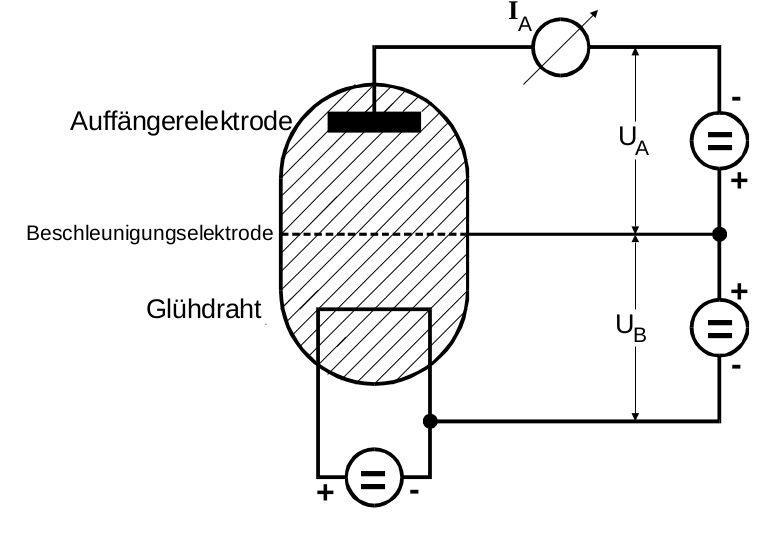
\includegraphics[scale=0.35]{schema.png}
  \caption{Der Aufbau des Franck-Hertz-Versuchs im Schema. \cite{anleitung}}
  \label{fig:1}
\end{figure}
Er besteht hauptsächlich aus einer evakuierten Glasröhre mit einem Tropfen Quecksilber
darin. Sobald das Quecksilber verdampft ist, stellt sich gemäß der Dampfdruckkurve
ein Gleichgewichtsdruck $p_\symup{sät}$ ein, der eine Temperaturabhängigkeit besitzt.
Somit kann durch Variation der Temperatur die Dampfdichte gesteuert werden. Ein Glühdraht
aus Wolfram wird eingeführt und erhitzt, bis sich durch den glühelektrischen Effekt
eine Elektronenwolke um den Draht gebildet hat. Gegenüber dem Drahlt liegt eine Netzelektrode,
an welche die positive Gleichspannung $U_B$ angelegt wird. DIe Elektronen werden nun auf
der Strecke zwischen Draht und Elektrode durch das elektrische Feld beschleunigt und erhalten die
Energie
\begin{equation*}
  \frac{m_0 \cdot v^2_\symup{vor}}{2} = e_0 \cdot U_B \, .
\end{equation*}
Dabei ist $e_0$ die Elementarladung. Hinter der Netzelektrode befindet sich eine Anode,
an der man den Auffängerstrom $I_A$ messen kann. Außerdem liegt im Vergleich zu
$U_B$ eine geringe Gegenspannung an. Das bedeutet, dass nur Elektronen, deren kinetische Energie
in Feldrichtung größer oder gleich $e_0 \cdot U_A$ ist, die Auffängerelektrode erreichen
können. \\
\\
Da sich aber sowohl zwischen Draht und Netzelektrode als auch zwischen
Netzelektrode und Auffängerelektrode noch die Quecksilberatome befinden, kommt es
zu Stößen. Dabei sind zwei Fälle zu unterscheiden:
\begin{itemize}
  \item Falls die Energie $U_B \cdot e_0$ gering ist finden nur elastische Stöße statt.
  Da die Massen der Stoßpartner so unterschiedlich groß sind, findet praktisch keine
  Energieübertragung statt. Allerdings ändert sich die Flugrichtung der Elektronen signifikant.

  \item Falls
  \begin{equation*}
    \frac{m_0 \cdot v^2_\symup{vor}}{2} \geq E_1 - E_0
  \end{equation*}
  gilt, dann wird das Quecksilberatom durch den Stoß mit dem Elektron angeregt.
  Es erhält die Energiedifferenz $E_1 - E_0$ und die Energie des Elektrons wird
  um den Betrag der Energiedifferenz verringert. Nach einer Relaxationszeit
  in der Größenordnung \SI{e-8}{\second} emmittiert das Quecksilberatom ein Photon
  mit der Frequenz
  \begin{equation*}
      h \nu = E_1 - E_0
  \end{equation*}
  und fällt in den Grundzustand zurück.
\end{itemize}

Die Anregung der Hg-Atome lässt sich über den Strom $I_A$ beobachten. Falls nämlich
$U_B$ ausgehend von 0 kontinuierlich erhöht wird, dann wird ab $U_B \geq U_A$ ein
Strom $I_A$ gemessen. Tritt bei weiterer Erhöhung der oben genannte zweite Fall ein,
also dass die kinetische Energie der Elektronen ein wenig größer oder gleich der Energiedifferenz
$E_1 - E_0$ wird, dann stoßen diese inelastisch und geben Energie ab. Damit fehlt ihnen
aber Energie, um das Gegenfeld $U_A$ zu überwinden und die Beschleunigungsstrecke ist ebenfalls
zu kurz, um die Elektronen auf die benötigte Geschwindigkeit zu beschleunigen. Somit
fällt der Strom an der Auffängerelektrode signifikant ab. Wird die Beschleunigungsspannung
aber weiter erhöht, können die Elektronen früher stoßen und haben danach noch genug Strecke,
um auf eine Geschwindigkeit zu beschleunigen, mit deren Hilfe das Gegenfeld $U_A$
überwunden werden kann. Somit steigt der Strom $I_A$ erneut.
Erreichen die Elektronen aber nach einem Stoß erneut die Energie
$E_1 - E_0$, so wird ein zweiter Stoß ausgeführt und der Strom sinkt wieder schlagartig
ab. In Abbildung \ref{fig:2} ist dieser Zusammenhang als Graph dargestellt.
\begin{figure}[h]
  \centering
  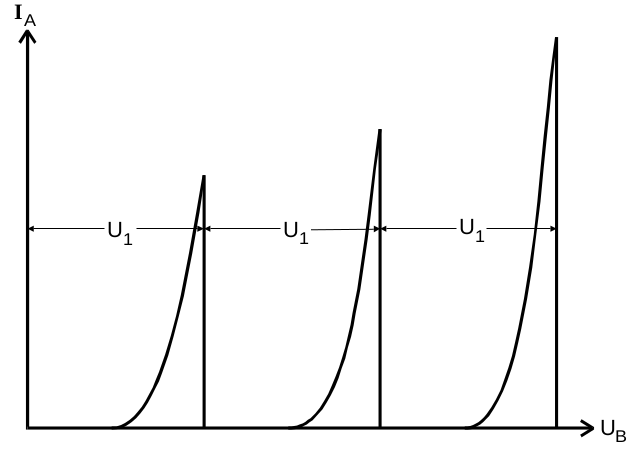
\includegraphics[scale=0.35]{strom.png}
  \caption{Der Strom $I_A$ gegen die Beschleunigungsspannung $U_B$ im Idealfall aufgetragen. \cite{anleitung}}
  \label{fig:2}
\end{figure}
Der Abstand $U_1$ zweier Maxima ergibt sich aus
\begin{equation}
  U_1 = \frac{1}{e_0} (E_1 - E_0) \, .
  \label{eqn:1}
\end{equation}

\subsection{Effekte mit Einfluss auf den Franck-Hertz-Versuch}
Die Kurve aus Abbildung \ref{fig:2} entspricht nicht den tatsächlichen Messergebnissen,
da im vorigen Kapitel nur der Idealfall betrachtet wurde. Folgende Effekte haben jedoch
einen Einfluss auf die Gestalt der Kurve:
\begin{itemize}
  \item Falls Glühdraht und Netzelektrode verschiedene Austrittsarbieten haben, was
  häufig der Fall ist, da der Glühdraht oft mit einer Metalllegierung ummantelt wird, dessen
  Austrittsarbeit niedriger liegt als die des Materials, aus dem die Glühkathode besteht,
  um bereits bei niedrigen Spannungen einen glühelektrischen Effekt zu erzielen, ist das
  Potential zwischen Draht und Elektrode verschieden von $U_B$.
  \begin{figure}[h]
    \centering
    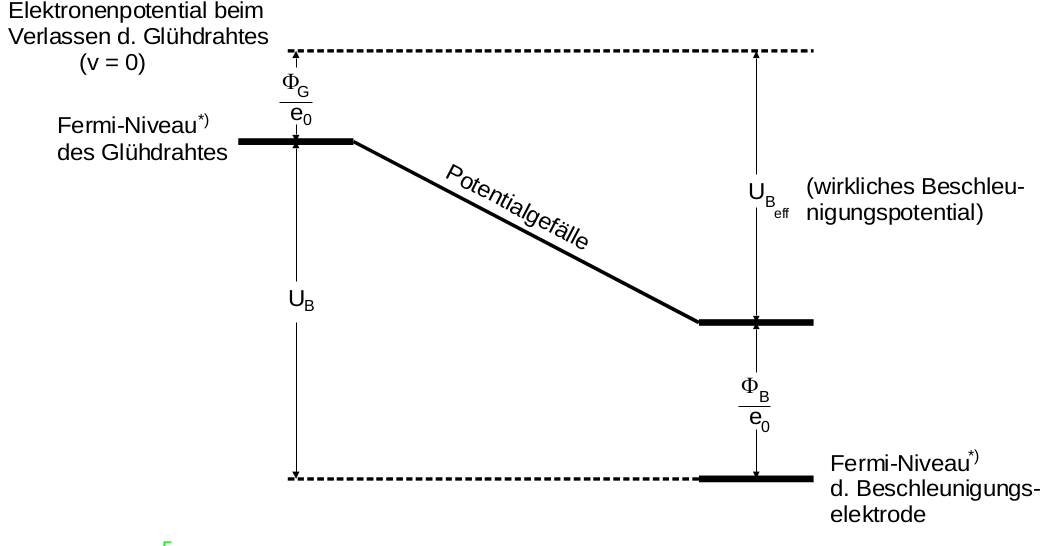
\includegraphics[scale=0.35]{pot.png}
    \caption{Potentialgefälle zwischen Draht und Elektrode. \cite{anleitung}}
    \label{fig:3}
  \end{figure}
  In Abbildung \ref{fig:3} sind die Verhältnisse dargestellt. Es ergibt sich
  \begin{equation}
    K = \frac{1}{e_0} (\Phi_B - \Phi_G)
    \label{eqn:2}
  \end{equation}
  als Audruck für das sogenannte Kontaktpotential. Die Franck-Hertz-Kurve ist um
  $K$ verschoben.

  \item Bisher ist davon ausgegnagen worden, dass alle Elektronen beim Anlegen der
  Beschleunigungsspannung eine Energie von 0 haben. Diese Annahme ist jedoch falsch,
  da die Elektronen aufgrund der Fermi-Dirac-Statistik bereits zufällig verteilte
  Energien besitzen. Das bedeutet, dass sie beim Stoß mit einem Quecksilberatom
  bereits eine höhere Geschwindigkeit besitzen, als sie eigentlich durch die Beschleunigungsspannung
  erhalten haben. Damit können die Elektronen nicht mehr nur bei einem bestimmten Spannungswert,
  sondern in einem endlichen Intervall inelastisch stoßen. Die Franck-Hertz-Kurve aus
  Abbildung \ref{fig:2} wird bei Annäherung an ein Maximum also ihren Anstieg verringern
  und danach stetig auf ein Minimum statt auf 0 fallen. Weiterhin spielen die elastische
  Stöße eine Rolle. Die Richtungsänderung ist irrelevant, falls der Stoß innerhalb der
  Beschleunigungsstrecke stattfindet, da das elektrische Feld die Elektronen wieder
  auf Kurs bringt, aber sobald ein elastischer Stoß im Gegenfeld geschieht, werden
  die Elektronen die Auffängerelektrode nicht mehr erreichen und die Franck-Hertz-Kurve
  sich verbreitern und abflachen.

  \item Damit die Elektronen mit den Hg-Atomen stoßen können, muss die mittlere freie Weglänge
  $\overline w$ der Atome gegenüber dem Anstand $a$ zwischen Draht und Elektrode um den
  Faktor 1000 bis 4000 kleiner sein. Die mittleren freie Weglänge lässt sich berechnen
  aus
  \begin{equation}
    \overline w = \num{0.0029}/p_\symup{sät}
    \label{eqn:3}
  \end{equation}
  mit
  \begin{equation}
    p_\symup{sät} = \num{5.5e7} \cdot \symup e^{-6876/T}
  \end{equation}
  mit $T$ als Temperatur. Somit gibt es wohl einen Temperaturbereich und damit auch
  einen Dampfdruckbereich, für die der Franck-Hertz-Effekt gut zu beobachten ist.
  Wird der Dampfdruckbereich unterschritten, wird die mittlere freie Weglänge größer
  und die Elektronen erreichen mit höherer Wahrscheinlichkeit die Auffängerelektrode ohne
  dabei zu stoßen. Wird $p_\symup{sät}$ zu groß, dann treten vermehrt elastische Stöße
  auf, die zu den bereits beschriebenen Richtungsänderungen führen. Damit sinkt die Anzahl
  der Elektronen, die die Auffängerelektrode erreichen können.
\end{itemize}

\section{Durchführung}
\subsection{Versuchsaufbau}
In Abbildung \ref{fig:4} ist der Schaltplan des Versuchsuafbaus zu sehen.
\begin{figure}
  \centering
  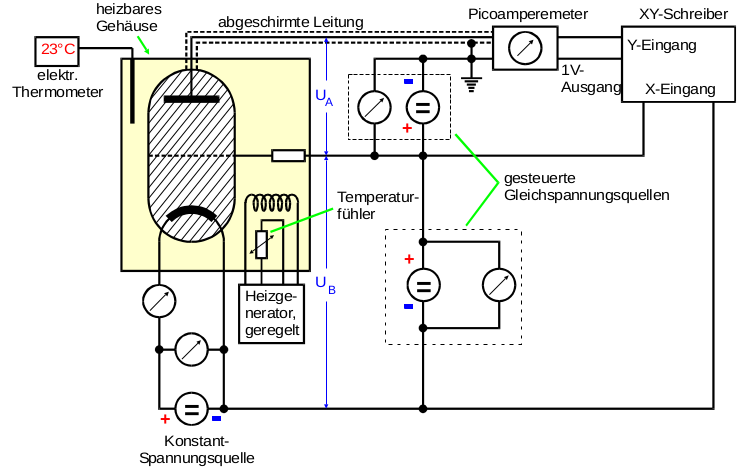
\includegraphics[scale=0.5]{aufbau.png}
  \caption{Schaltplan des Versuchsaufbaus. \cite{anleitung}}
  \label{fig:4}
\end{figure}
Er besteht im Wesentlichen aus der bereits beschrieben Glasröhre mit den angelegten
Spannungen $0 \leq U_B \leq \SI{60}{\volt}$ und $0 \leq U_A \leq \SI{11}{\volt}$, die
über ein Konstantspannungsgerät geliefert werden.
Die Temperatur kann mithilfe des regelbaren Heizgenerators eingestellt werden,
der das Blechgehäuse um die Glasröhre heizt.
Die aktuelle
Temperatur wird über einen Temperaturfühler abgelesen. Der Auffängerstrom $I_A$ wird über das
Picomaperemeter abgelesen. Über den XY-Schreiber lassen sich $I_A$ und wahlweise $U_A$ oder
$U_B$ gegeneinander auftragen.

\subsection{Versuchsdurchführung}
Zuerst wird der Auffängerstrom $I_A$ bei konstantem $U_B$ in Abhängigkeit von $U_A$
gemessen. Dafür wird der XY-Schreiber so präpariert, dass $U_A$ auf der x- und $I_A$
auf der y-Achse liegt. Sodann wird bei $U_B = \SI{11}{\volt}$ bzw. $\SI{10}{\volt}$
und bei Zimmertemperatur $U_A$ von 0 bis \SI{11}{\volt} gesteigert und $U_A$ gegen
$I_A$ vom XY-Schreiber aufgetragen. Zum Schluss wird der Plot noch mit einer \SI{1}{\volt}-Skala
versehen und die Messung bei ca. \SI{150}{\celsius} wiederholt. \\
\\
Danach wird die Apparatur auf ca. \SI{105}{\celsius} erhitzt und diesmal bei konstantem
$U_A = \SI{-30}{\volt}$ die Beschleunigungsspannung über den angegebenen Bereich varriert
und der Auffängerstrom $I_A$ gegen die Beschleunigungsspannung vom XY-Schreiber aufgetragen. \\
\\
Zum Schluss werden bei $T = \SI{160}{\celsius}, \SI{170}{\celsius}, \SI{180}{\celsius}, \SI{190}{\celsius}$ und $\SI{200}{\celsius}$ Franck-Hertz-Kurven
bei einer konstanten Gegenspannung von \SI{-1}{\volt} aufgenommen, indem wieder $I_A$ gegen
$U_B$ aufgetragen wird.

\section{Auswertung}
\subsection{Fehlerrechnung}
\label{Fehler}
Für die Fehlerrechnung gibt:
\begin{equation}
  \overline{T} = \frac{1}{n} \sum_{i=1}^{n} T_{i}
\end{equation}
den Mittelwert, sowie:
\begin{equation}
  \sigma_{\overline{T}} = \sqrt{\frac{1}{n(n-1)} \sum_{i=1}^{n}(\overline{T}-T_i)^2}
\end{equation}
den Fehler des Mittelwertes.
In Fällen, in denen fehlerbehaftete Größen in einer Gleichung zur Bestimmung
einer anderen Größe verwendung finden, wird der resultierende Fehler durch
$\textsc{uncertainties}$ in $\textsc{python}$ berechnet.
\subsection{Bestimmen der Umrechnungsfaktoren der U-Achsen}
\label{Umrechnung}
Zuerst werden für alle Messreihen die Skalierungsfaktoren der $U$-Achsen bestimmt,
um die Messwerte von \si{\milli\metre} in \si{\volt} umzurechnen. Dafür werden
die Abstände der einzellnen Skalenpunkte zum Nullpunkt gemessen und durch die
Funktion $\textsc{curve-fit}$ aus dem Paket
$\textsc{optimize}$ in $\textsc{python-scipy}$ mit einer linearen Funktion
\begin{equation*}
  U(x) = m \cdot x + n
\end{equation*}
gefittet. In Tabelle \ref{tab:1} finden sich die Abstände aller Skalenpunkte,
In Tabelle \ref{tab:2} die Parameter der Umrechnungsfunktion. Die aus der Regression
folgenden Fehler sind, insbesondere bei den für die Umrechnung wichtigen Geradensteigungen,
so klein das sie weitaus geringer als die bestmögliche Ablesegenauigkeit auf dem Millimeterpapier
sind. Die Fehler werden daher vernachlässigt.
\begin{table}
  \centering
  \caption{Abstände der Skalenpunkte vom Nullpunkt}
  \label{tab:1}
  \begin{tabular}{S S | S S | S S | S S}
    \toprule
    \multicolumn {2}{c}{$T \approx \SI{20}{\celsius}$} &
    \multicolumn {2}{c}{$T = \SI{152}{\celsius}$} &
    \multicolumn {2}{c}{Franck-Hertz-Kurve} &
    \multicolumn {2}{c}{Ionisierung} \\
    $U/$\si{\volt} & $x/$\si{\milli\metre} & $U/$\si{\volt} & $x/$\si{\milli\metre} &
    $U/$\SI{5}{\volt} & $x/$\si{\milli\metre} & $U/$\SI{5}{\volt} & $x/$\si{\milli\metre} \\
    \midrule
    1 & 21 & 1 & 19 & 1 & 22 & 1 & 35 \\
    2 & 39 & 2 & 39 & 2 & 42 & 2 & 71 \\
    3 & 58 & 3 & 56 & 3 & 61 & 3 & 105 \\
    4 & 76 & 4 & 76 & 4 & 79 & 4 & 140 \\
    5 & 84 & 5 & 95 & 5 & 98 & 5 & 174 \\
    6 & 103 & 6 & 114 & 6 & 118 & 6 & 215 \\
    7 & 123 & 7 & 133 & 7 & 136 & & \\
    8 & 143 & 8 & 163 & 8 & 154 & & \\
    9 & 160 & 9 & 172 & 9 & 171 & & \\
    10 & 184 & 10 & 192 & 10 & 190 & & \\
    11 & 199 & 11 & 208 & 11 & 209 & & \\
    \bottomrule
  \end{tabular}
\end{table}
\begin{table}
  \centering
  \caption{Parameter der Umrechnungsfunktion}
  \label{tab:2}
  \begin{tabular}{c | c  c  c  c}
    \toprule
    Messreihe &
    $T \approx \SI{20}{\celsius}$ &
    $T = \SI{152}{\celsius}$ &
    Franck-Hertz-Kurve &
    Ionisierung \\
    \midrule
    $m/$\si[per-mode=reciprocal]{\volt\per\milli\metre} &  0.0560 & 0.0519 &  0.2662 & 0.1411 \\
    $n/$\si[per-mode=reciprocal]{\volt} & -0.0576 & 0.0218 & -0.8909 & 0.0884 \\
    \bottomrule
  \end{tabular}
\end{table}
\subsection{Betrachtung der differentiellen Energieverteilung}
Die aus den erhaltenen integralen Energieverteilungen durch Anlegen von Steigungsdreiecken
in \SI{5}{\milli\metre}-Schritten nach $m_{\symup{mom}} = \symup{\Delta}y / \symup{\Delta}x$
erhaltenen Momentansteigungen finden sich in Tabelle \ref{tab:3}. Auftragen der Momentansteigungen
in nach Abschnitt \ref{Umrechnung} umgerechneten \SI{5}{\milli\metre}-Schritten liefert
die Abbildungen \ref{Abb:1} ($T \approx \SI{20}{\celsius}$) und \ref{Abb:2} ($T = \SI{152}{\celsius}$)
daregstellten Näherungen für die Ableitung der integralen Energieverteilung, also
eine Näherung für die differntielle Energieverteilung.
\begin{table}
  \centering
  \caption{Kantenlängen der Steigungsdreiecke sowie daraus berechnete Momentansteigungen.
  $\symup{\Delta}x$ beträgt jeweils \SI{5}{\milli\metre}.}
  \label{tab:3}
  \begin{tabular}{S S | S S || S S | S S}
    \toprule
    \multicolumn {4}{c}{$T \approx \SI{20}{\celsius}$} &
    \multicolumn {4}{c}{$T = \SI{152}{\celsius}$} \\
    $\symup{\Delta}y$ & $m_{\symup{mom}}$ &
    $\symup{\Delta}y$ & $m_{\symup{mom}}$ &
    $\symup{\Delta}y$ & $m_{\symup{mom}}$ &
    $\symup{\Delta}y$ & $m_{\symup{mom}}$ \\
    \midrule
    0.50 & 2.246 & 2.50 & 11.230 & 15.500 & 55.125 & 3.000 & 10.669 \\
    0.50 & 2.246 & 2.00 & 8.984  & 14.500 & 51.568 & 2.500 & 8.891 \\
    0.50 & 2.246 & 2.50 & 11.230 & 10.000 & 35.564 & 0.035 & 0.124 \\
    0.50 & 2.246 & 3.00 & 13.476 & 13.000 & 46.234 & 0.035 & 0.124 \\
    0.75 & 3.369 & 5.00 & 22.461 & 6.000 & 21.339 & 0.035 & 0.124 \\
    0.75 & 3.369 & 5.50 & 24.707 & 2.000 &  7.113 & 0.035 & 0.124 \\
    0.75 & 3.369 & 7.00 & 31.445 & 2.000 &  7.113 & 0.035 & 0.124 \\
    0.75 & 3.369 & 8.50 & 38.183 & 4.000 & 14.226 & 0.035 & 0.124 \\
    1.00 & 4.492 & 16.50 &  74.120 & 4.500 & 16.004 & 0.035 & 0.124 \\
    1.00 & 4.492 & 50.00 & 224.606 & 5.000 & 17.782 & 0.035 & 0.124 \\
    1.00 & 4.492 & 23.00 & 103.319 & 5.500 & 19.560 & 0.035 & 0.124 \\
    1.00 & 4.492 & 2.00 & 8.984 & 6.000 & 21.339 & 0.035 & 0.124 \\
    1.00 & 4.492 & 0 & 0 & 6.000 & 21.339 & 0.035 & 0.124 \\
    1.00 & 4.492 & 0 & 0 & 7.000 & 24.895 & 0.035 & 0.124 \\
    1.00 & 4.492 & 0 & 0 & 7.500 & 26.673 & 0.035 & 0.124 \\
    1.00 & 4.492 & 0 & 0 & 6.000 & 21.339 & 0.035 & 0.124 \\
    1.50 & 6.738 & 0 & 0 & 6.000 & 21.339 & 0.035 & 0.124 \\
    1.00 & 4.492 & 0 & 0 & 7.000 & 24.895 & 0.035 & 0.124 \\
    2.00 & 8.984 & 0 & 0 & 6.000 & 21.339 & 0.035 & 0.124 \\
    1.50 & 6.738 & 0 & 0 & 7.000 & 24.895 & 0.035 & 0.124 \\
    2.00 & 8.984 &  &  & 5.000 & 17.782 &  &  \\
    \bottomrule
  \end{tabular}
\end{table}
\begin{figure}
  \centering
  \subcaptionbox{$T \approx \SI{20}{\celsius}$ \label{abb:1}}[0.49\textwidth]{
    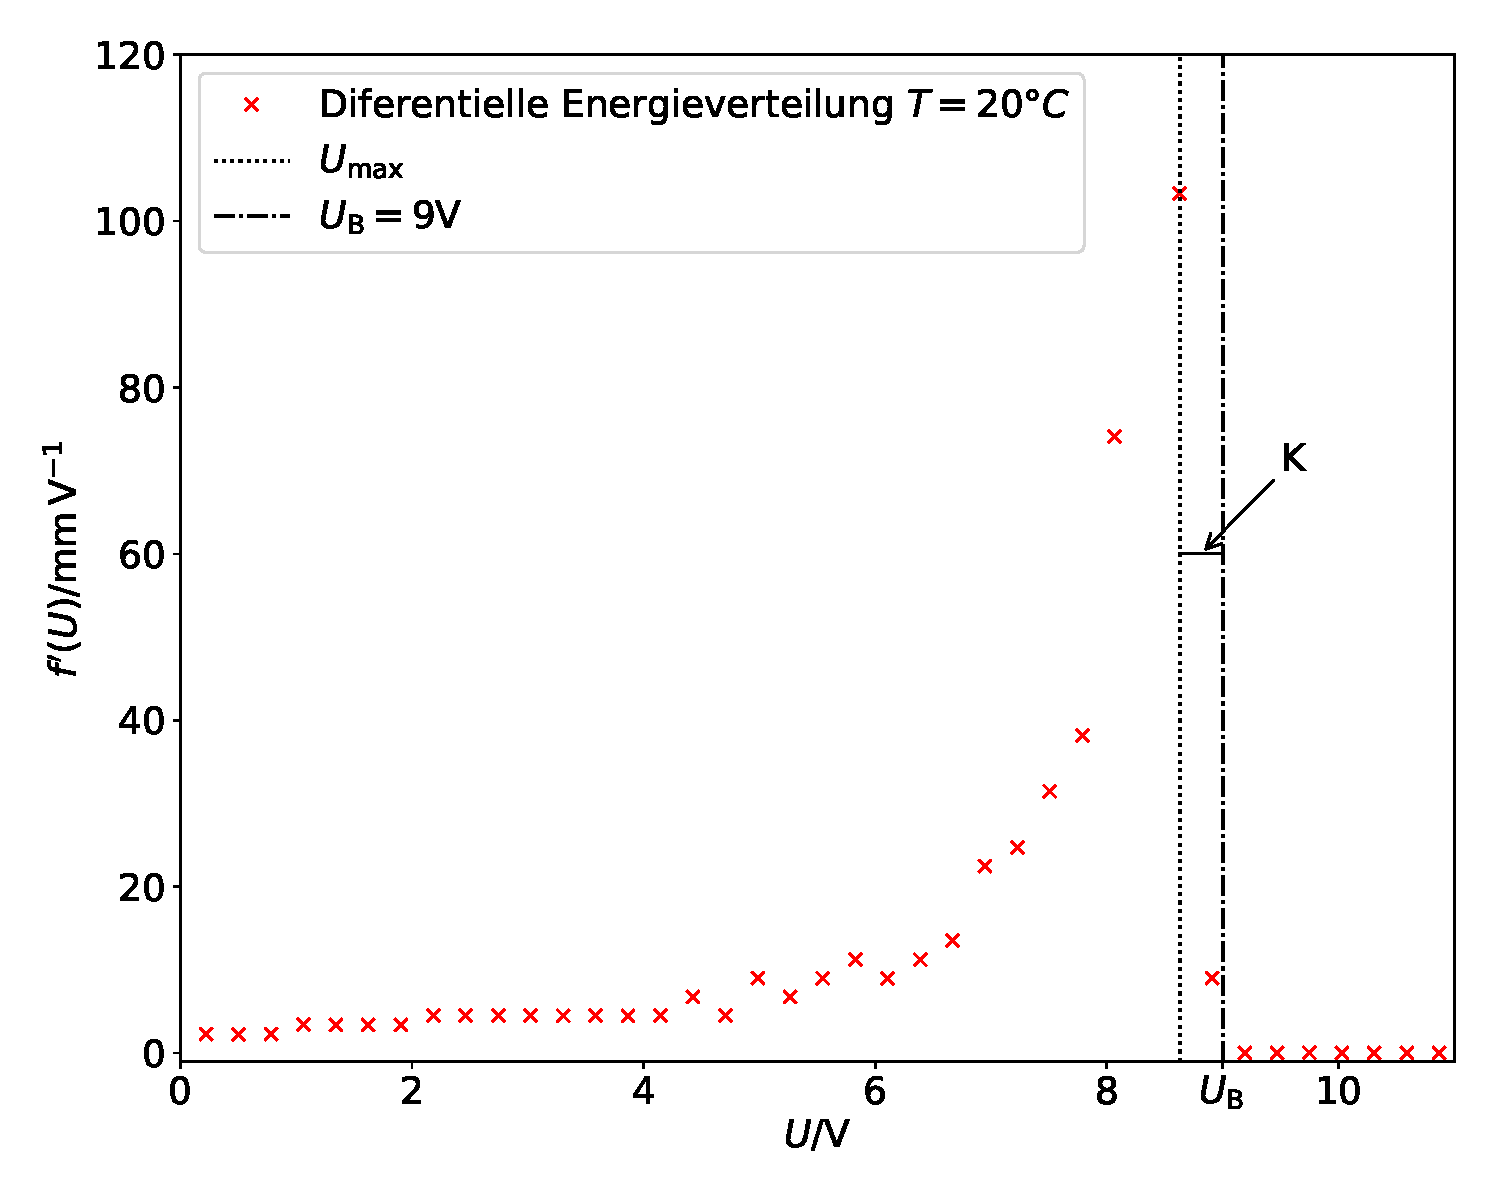
\includegraphics[width=0.49\textwidth]{T20.pdf}
    }
  \hfill
  \subcaptionbox{$T = \SI{152}{\celsius}$ \label{abb:2}}[0.49\textwidth]{
    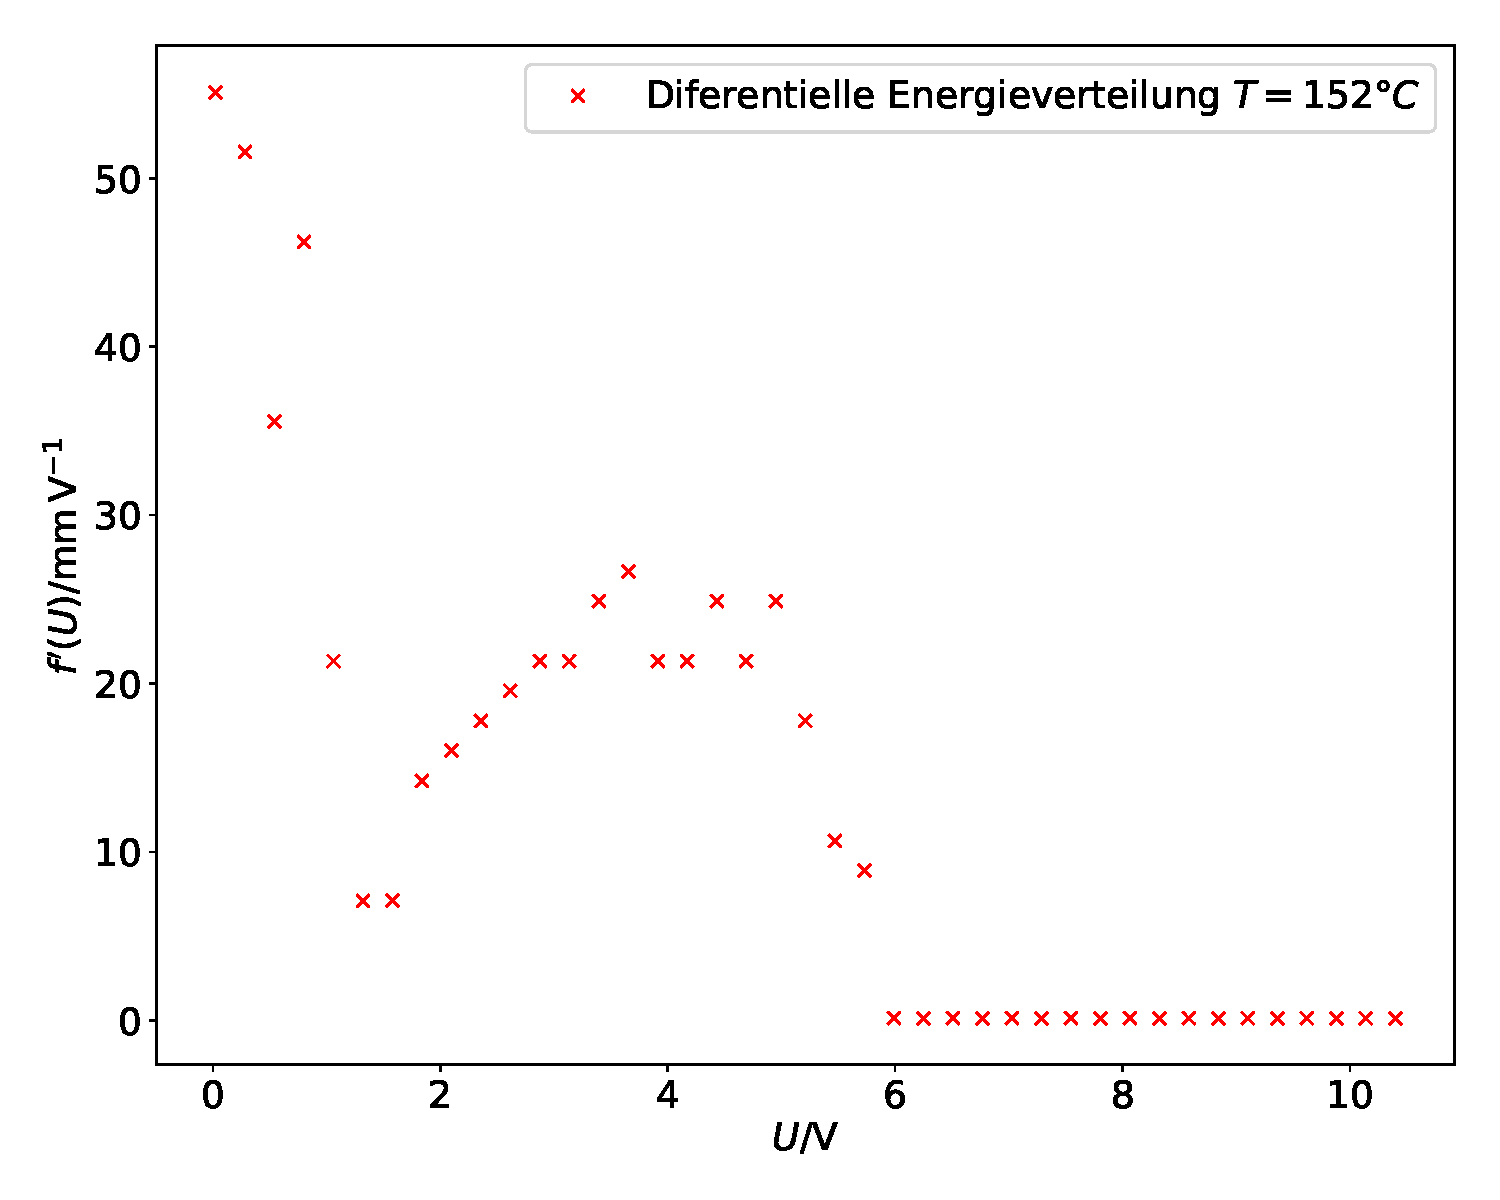
\includegraphics[width=0.49\textwidth]{T152.pdf}
    }
  \hfill
  \caption{Näherungsweise differentielle Energieverteilungen.}
\end{figure}
In Abbildung \ref{abb:1} ist gut der nach der $\textsc{Fermi-Dirac}$-Statistik
zu erwartende breite Peak zu sehen. Das Maximum des Peaks liegt bei \SI{8.63}{\volt}.
Aus der Differenz zwischen Beschleunigungsspannung $U_{\symup{B}} = \SI{9}{\volt}$
und dem Maximum folgt für das Kontaktpotential ein Wert von:
\begin{equation*}
  K_1 = \SI{0.37}{\volt}.
\end{equation*}
Die Abweichung zwischen den Abbildungen \ref{abb:1} und \ref{abb:2} lassen sich dadurch
erklären, dass bei der deutlich höheren Temperatur von $T = \SI{152}{\celsius}$ die mittlere
freie Weglänge stark abnimmt, sodass es zu mehr Stößen kommt.
\subsection{Auswertung der Frack-Hertz Kurve}
Die Abstände zwischen zwei Maxima sind in Tabelle \ref{tab:4} angegeben. Mittelwertbildung
nach den in Kapitel \ref{Fehler} aufgeführten Formeln liefert zusammen mit den in Kapitel
\ref{Umrechnung} errechneten Zusammenhängen einen Wert von
\begin{equation*}
  \symup{\Delta}E = \SI{3.93(7)}{\electronvolt}
\end{equation*}
für die Anregungsenergie von Quecksilber. Diese Energie entspricht einer Wellenlänge
von
\begin{equation*}
  \lambda = \SI{316(6)}{\nano\metre},
\end{equation*}
also einer Wellenlänge im bereich des UV-Lichtes. Zwischen dem erstem Maximum und dem
Nullpunkt der Messung muss zusätzlich zur Anregungsenergie noch das Kontaktpotential überwunden werden.
Aus der Differenz zwischen $U$-Wert des ersten Maximums (\SI{4.97}{\volt}) und der oben
bestimmten Anregungsenergie folgt für das Kontaktpotential ein Wert von:
\begin{equation*}
  K_2 = \SI{1.04(7)}{\volt}
\end{equation*}
\begin{table}
  \centering
  \caption{Abstände zwischen 2 Maxima.}
  \label{tab:4}
  \begin{tabular}{c c}
    \toprule
    Nr. & $\symup{\Delta}x/$\si{\milli\metre}\\
    \midrule
    1 & 17 \\
    2 & 17 \\
    3 & 18 \\
    4 & 19 \\
    5 & 18 \\
    6 & 18 \\
    7 & 19 \\
    8 & 19 \\
    9 & 18 \\
    \bottomrule
  \end{tabular}
\end{table}
\subsection{Auswertung der Ionisierungskurve}
Die aus der Ionisierungskurve entnommene und hier beachteten Messwertpaare
finden sich in Tabelle \ref{tab:5}. Eine lineare Regression durch die nicht Umgerechneten
Werte wie in Kapitel \ref{Umrechnung} liefert für die Regressionsgerade:
\begin{align*}
  m &= \num{1.46(4)} \\
  n &= \SI{-144(7)}{\milli\metre}.
\end{align*}
Aus dem Schnittpunkt der Gerade mit der $x$-Achse sowie nach Umrechnung folgt für
$U_\symup{Ion}+\bar{K} = -n/m$:
\begin{equation*}
  U_\symup{Ion}+\bar{K} = \SI{14.1(8)}{\volt}.
\end{equation*}
Subtraktion mit dem Mittelwert der vorher bestimmten Werte für $K$ von
$\bar{K} = \SI{0.703(35)}{\volt}$ liefert:
\begin{equation*}
  U_\symup{Ion} = \SI{13.3(8)}{\electronvolt}.
\end{equation*}
Die Regression findet sich in Abbildung \ref{abb:3}.
\begin{figure}
  \centering
  \subcaptionbox{Grafische Darstellung mit Regression \label{abb:3}}[0.7\textwidth]{
    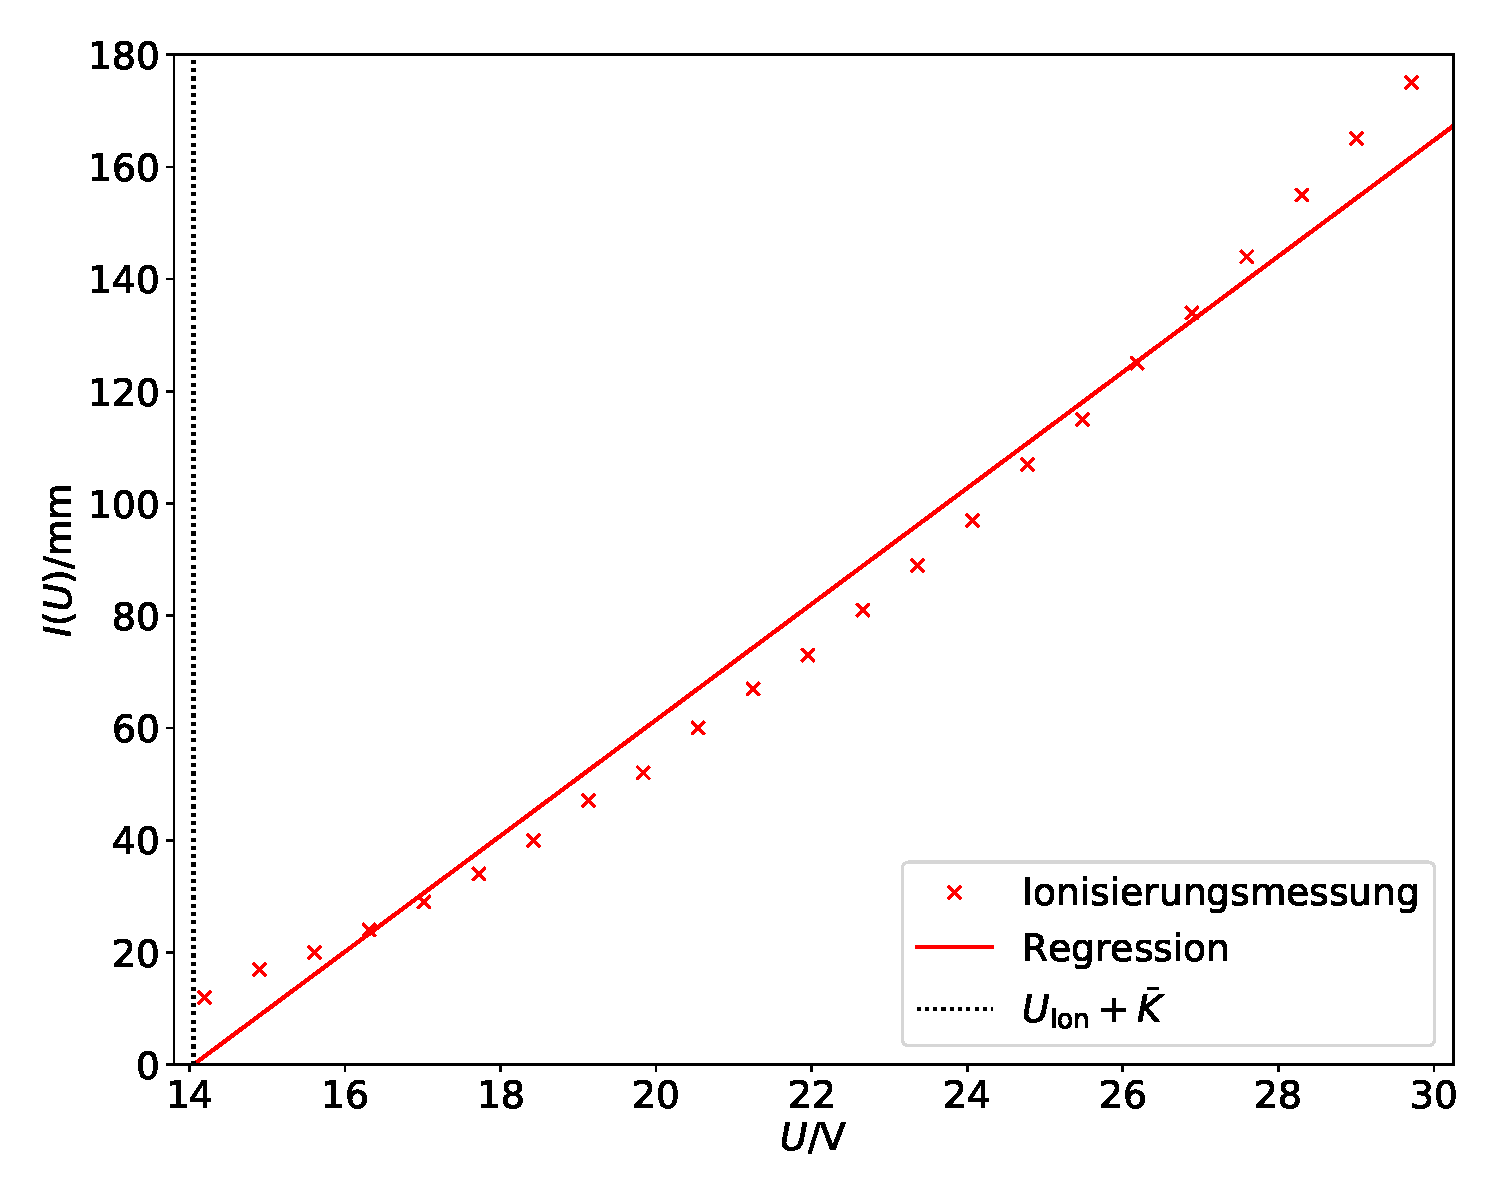
\includegraphics[width=0.7\textwidth]{Ion.pdf}
    }
  \hfill
  \subcaptionbox{Messwertpaare \label{tab:5}}[0.29\textwidth]{
    \begin{tabular}{c c}
      \toprule
      $x/$\si{\milli\metre} & $y/$\si{\milli\metre}\\
      \midrule
      95 & 4 \\
      100 & 7 \\
      105 & 12 \\
      110 & 15 \\
      115 & 19 \\
      120 & 24 \\
      125 & 29 \\
      130 & 35 \\
      135 & 42 \\
      140 & 47 \\
      145 & 55 \\
      150 & 62 \\
      155 & 68 \\
      160 & 76 \\
      165 & 84 \\
      170 & 92 \\
      175 & 102 \\
      180 & 110 \\
      185 & 120 \\
      190 & 129 \\
      195 & 139 \\
      200 & 150 \\
      205 & 160 \\
      210 & 170 \\
      \bottomrule
    \end{tabular}
    }
  \hfill
  \caption{Ionisierungsmessung.}
\end{figure}
\section{Diskussion}
Im Vergleich zwischen dem bestimmten Wert von \SI{3.93(7)}{\electronvolt} und dem
Literaturwert von \SI{4.9}{\electronvolt}\cite{Anregungsenergie} fällt eine Große
Abweichung auf. Der Literaturwert befindet sich in einer 14-$\sigma$ Umgebung
um den Experimentell bestimmten Wert. Es ist also mit starken systematischen Fehlern
zu rechnen. Wahrscheinlichste Fehlerquelle ist hierbei das Voltmeter des Spannungsgerätes
des Beschleunigungsstroms. Hier wurde als maximaler Wert ca. \SI{55}{\volt} angezeigt,
das Gerät ließ sich auch im Gegensatz zu den anderen Voltmetern nicht über die Skalengrenze
übersteuern. Es liegt damit der Schluss nahe, dass das Voltmeter einen zu geringen
Wert angezeigt hat. Tatächlich führt eine Betrachtung eines höheren Maximalspannungswertes
und damit einer geänderten Achsenskalierung zu einem weitaus besseren Wert für die
Anregungsenergie.\\
\noindent
Bei der Betrachtung der Ionisierungsmessung liegt der Literaturwert von
\SI{10.438}{\electronvolt} \cite{Ionisierungsenergie}
hingegen in einer 4-$\sigma$ Umgebung um den experimentell Bestimmten Wert von
\SI{13.3(8)}{\electronvolt}.
Problematisch war hier das Festlegen des Intervalls der Messwerte, durch die die Sekante
gelegt werden kann. Ein hinzunehmen weiterer Messwert in Richtung Nullpunkt könnte den
Wert dem Literaturwert annähern, ist aber zunehmend schwer zu Rechtfertigen. Auch ist
hier wahrscheinlich, dass die gleichen Fehler wie bei der Messung der Anregungsenergie
auftreten. Generell sollte das Experiment zur Verifizierung der Messwerte mit einem
anderen Spannungsgerät widerholt werden. Problematisch gestaltete sich in allen
unter Beheizung durchgeführten Versuchsteilen ein Konstanthalten der Temperatur
im Aufbau, daher ist auch hier mit systematischen Fehlern zu rechnen.
Ein Gerät das eine konstante Heizung ermöglicht könnte die Messgenauigkeit stark
erhöhen.
\newpage
\nocite{*}
\printbibliography
